\documentclass[13pt,a4paper,oneside]{book} % twoside for draft

% Packages
% Font
\usepackage{times}%
\usepackage{pifont}%
\usepackage[utf8]{inputenc}
\usepackage[T5]{fontenc}  % T5 encoding for Vietnamese

% Vietnamese language support
\usepackage[vietnamese,english]{babel}
\selectlanguage{english}  % Default to English, switch to Vietnamese when needed

% Figure
\usepackage{graphicx}%
\usepackage[font=normalsize,labelfont=bf]{caption}
\usepackage{subcaption}

% Math
\usepackage{amsmath,amssymb,amsfonts}%
\usepackage{amsthm}%
\usepackage{mathrsfs}%

% Table
\usepackage{multicol}%
\usepackage{multirow}%
\usepackage{adjustbox}%

% Color
\usepackage{xcolor}%
\usepackage{colortbl}%

% Text
\usepackage{textcomp}%
\usepackage[normalem]{ulem}%

% Algorithm
% \usepackage[linesnumbered, ruled, vlined]{algorithm2e}%
\usepackage[chapter]{algorithm}% number algorithms per chapter (Giải thuật 2.1, 4.1, ...)
\usepackage{algorithmicx}%
\usepackage{algpseudocode}%

\usepackage{tcolorbox}
\tcbuselibrary{theorems}

\newcounter{lemma}
\newcounter{property}
\newcounter{theorem}

\newtcbtheorem[use counter=lemma]{lemma}{Lemma}{
  colback=white,
  colframe=black,
  fonttitle=\bfseries,
  boxrule=0.8pt,
  arc=0mm,
}{lem}

\newtcbtheorem[use counter=property]{property}{Property}{
  colback=white,
  colframe=black,
  fonttitle=\bfseries,
  boxrule=0.8pt,
  arc=0mm,
}{prob}

\newtcbtheorem[use counter=theorem]{theorem}{Theorem}{
  colback=white,
  colframe=black,
  fonttitle=\bfseries,
  boxrule=0.8pt,
  arc=0mm,
}{theo}

% Appendix
\usepackage[title]{appendix}%
\renewcommand{\appendixname}{Appendix}
\renewcommand{\appendixtocname}{Appendix}

% Format
\usepackage[top=3cm, bottom=3cm, left=3.5cm, right=2cm]{geometry}
\usepackage{setspace}

\usepackage{tocloft}
% \renewcommand{\contentsname}{\centering Contents}

\usepackage[hypertexnames=false]{hyperref}
\usepackage{ragged2e}  % đặt ở preamble

% sectsty must load BEFORE titlesec: it redefines the sectioning internals and
% would silently wipe every \titleformat below (sections were falling back to
% the 10pt class defaults). It stays only for \chapterfont, which titlesec
% leaves alone.
\usepackage{sectsty}
\chapterfont{\centering\MakeUppercase}

% NOTE: no [explicit] option -- with it, the title only prints where #1 appears
% in the last \titleformat argument, and these blocks leave it empty, which
% silently drops every heading's text.
\usepackage{titlesec}
\titleformat{\section}       % command to redefine
  {\fontsize{16pt}{19pt}\selectfont\bfseries}          % format: size + bold
  {\thesection}              % label
  {1em}                      % spacing between label and title
  {}                         % code before title (empty here)

\titleformat{\subsection}
  {\fontsize{14pt}{17pt}\selectfont\bfseries}          % between body (13pt) and section (16pt)
  {\thesubsection}
  {1em}
  {}

% Without an explicit size the class default leaves subsubsection at 10pt
% (book has no real 13pt option), smaller than the body text.
\titleformat{\subsubsection}
  {\fontsize{13pt}{15pt}\selectfont\bfseries}          % body size, bold
  {\thesubsubsection}
  {1em}
  {}

\usepackage{fancyhdr}
\pagestyle{fancy}

% Page number
\fancyhf{} % clear header/footer
\fancyhead[C]{\normalsize \thepage} % page number top center
\renewcommand{\headrulewidth}{0pt}
% Also fix the 'plain' style used on some pages (e.g., chapter pages)
\fancypagestyle{plain}{
    \fancyhf{}
    \fancyhead[C]{\normalsize \thepage}
    \renewcommand{\headrulewidth}{0pt}
}

% Bold \fbox
\setlength{\fboxrule}{2pt}

% Others
% \usepackage{arydshln}%
\usepackage{booktabs}%
\usepackage{manyfoot}%
\usepackage{listings}%
\usepackage[symbol]{footmisc}%
\usepackage{bbm}%
\usepackage{pdflscape}
% (sectsty moved above titlesec -- see the section-format block.)
\usepackage{caption}
\DeclareCaptionLabelSeparator{customspace}{\hspace{0.2cm}}
\captionsetup{labelsep=customspace}

% Packages from original thesis
\usepackage{longtable}
\usepackage{threeparttable}
\usepackage{float}
\usepackage{enumitem}
\usepackage{indentfirst}
\usepackage{anyfontsize}
\usepackage{chngcntr}
\usepackage{tikz}
\usetikzlibrary{positioning, shapes.geometric, arrows.meta, fit}

% Loaded at the very end to prevent conflict with other table packages
\usepackage{arydshln}

\input{setup/math_commands}
\usepackage{setup/macros}
% \usepackage[style=ieee]{biblatex}
% \addbibresource{main.bib}

% Hyperref settings
\hypersetup{
    colorlinks=true,
    linkcolor=black,
    filecolor=black,      
    urlcolor=black,
    citecolor=black,
    pdftitle={Master's Thesis},
    pdfauthor={Lê Phúc Đức},
}

% Page layout - 1.5 line spacing, normal character spacing
\onehalfspacing
\setlength{\parindent}{1cm}

% Personal information (customize these)
% Vietnamese forms are the ones printed on the official pages (cover, committee
% page, task sheet, ly lich trich ngang); the English ones are used on the
% courtesy English task sheet and the English abstract.
\newcommand{\thesistitlevn}{NGHIÊN CỨU VÀ PHÁT TRIỂN HỆ THỐNG TỰ ĐỘNG PHÁT HIỆN HIỆN TƯỢNG TRÔI DẠT VÀ CẬP NHẬT MÔ HÌNH HỌC MÁY THÍCH ỨNG}
\newcommand{\thesistitle}{RESEARCH AND DEVELOPMENT OF AN ADAPTIVE MACHINE LEARNING SYSTEM\\WITH AUTOMATIC CONCEPT DRIFT DETECTION AND MODEL UPDATING}
\newcommand{\studentname}{LÊ PHÚC ĐỨC}
\newcommand{\studentid}{2370116} % Add student ID here
\newcommand{\majorvn}{Khoa học máy tính}
\newcommand{\major}{Computer Science}
\newcommand{\majorcode}{8480101}
\newcommand{\supervisorone}{PGS.~TS.~\textbf{Thoại Nam}}
\newcommand{\supervisortwo}{TS.~\textbf{Nguyễn Quang Hùng}}
\newcommand{\supervisoroneen}{Assoc.~Prof.~Dr.~\textbf{Thoại Nam}}
\newcommand{\supervisortwoen}{Dr.~\textbf{Nguyễn Quang Hùng}}
% TODO fill in once the defence is scheduled; BIEU MAU 4 wants "ngay ... thang ... nam ..."
\newcommand{\defensedate}{ngày 17 tháng 6 năm 2026}
\newcommand{\submissiondatevn}{tháng 5 năm 2026}
\newcommand{\submissiondate}{May 2026}

\begin{document}

% Vietnamese names for the structural elements. The thesis is written in
% Vietnamese, so the furniture follows suit; BIEU MAU 4 names these sections
% in Vietnamese ("Muc luc", "Tai lieu tham khao", ...).
\renewcommand{\chaptername}{CHƯƠNG}
\renewcommand{\tablename}{Bảng}
\renewcommand{\figurename}{Hình}
\floatname{algorithm}{Giải thuật}
\renewcommand{\bibname}{TÀI LIỆU THAM KHẢO}
\renewcommand{\appendixname}{Phụ lục}

% Page order per BIEU MAU 4: cover (twice), committee page, task sheet.
\newpage

% =============================================================================
% Trang bia / trang 1, reproduced from BIEU MAU 4. The form prints this page
% verbatim with point sizes attached, so the wording and the sizes below are
% taken directly from it:
%     DAI HOC QUOC GIA THANH PHO HO CHI MINH   (size 12)
%     TRUONG DAI HOC BACH KHOA                 (size 13)
%     --------------------
%     HO VA TEN HOC VIEN                       (size 16)
%     TEN DE TAI                               (size 20)
%     Chuyen nganh: / Ma nganh:                (size 16)
%     LUAN VAN THAC SI                         (size 20)
%     Thanh pho Ho Chi Minh, thang ... nam ... (size 13)
% =============================================================================

\begin{titlepage}
    \centering

    % Box around entire page content
    \fbox{
    \begin{minipage}[t][0.9\textheight]{0.95\textwidth}
        \vspace{1cm}
        \begin{center}
            {\fontsize{12pt}{14pt}\selectfont ĐẠI HỌC QUỐC GIA THÀNH PHỐ HỒ CHÍ MINH}

            \vspace{2mm}

            {\fontsize{13pt}{15pt}\selectfont \textbf{TRƯỜNG ĐẠI HỌC BÁCH KHOA}}

            \vspace{2mm}

            \rule{4cm}{0.4pt}

            \vspace{2cm}

            {\fontsize{16pt}{19pt}\selectfont \textbf{\studentname}}

            \vspace{2.5cm}

            % Title
            \parbox{0.85\textwidth}{\centering \fontsize{20pt}{24pt}\selectfont \bfseries \thesistitlevn \par}

            \vfill

            \begin{flushleft}
            \hspace*{4cm}{\fontsize{16pt}{19pt}\selectfont Chuyên ngành: \majorvn}

            \vspace{1mm}

            \hspace*{4cm}{\fontsize{16pt}{19pt}\selectfont Mã ngành: \majorcode}
            \end{flushleft}

            \vspace{1.5cm}

            {\fontsize{20pt}{24pt}\selectfont \textbf{LUẬN VĂN THẠC SĨ}}

            \vfill

            {\fontsize{13pt}{15pt}\selectfont Thành phố Hồ Chí Minh, \submissiondatevn}

            \vspace{0.5cm}
        \end{center}
    \end{minipage}
    }
\end{titlepage}

\newpage

% =============================================================================
% Trang bia / trang 1, reproduced from BIEU MAU 4. The form prints this page
% verbatim with point sizes attached, so the wording and the sizes below are
% taken directly from it:
%     DAI HOC QUOC GIA THANH PHO HO CHI MINH   (size 12)
%     TRUONG DAI HOC BACH KHOA                 (size 13)
%     --------------------
%     HO VA TEN HOC VIEN                       (size 16)
%     TEN DE TAI                               (size 20)
%     Chuyen nganh: / Ma nganh:                (size 16)
%     LUAN VAN THAC SI                         (size 20)
%     Thanh pho Ho Chi Minh, thang ... nam ... (size 13)
% =============================================================================

\begin{titlepage}
    \centering

    % Box around entire page content
    \fbox{
    \begin{minipage}[t][0.9\textheight]{0.95\textwidth}
        \vspace{1cm}
        \begin{center}
            {\fontsize{12pt}{14pt}\selectfont ĐẠI HỌC QUỐC GIA THÀNH PHỐ HỒ CHÍ MINH}

            \vspace{2mm}

            {\fontsize{13pt}{15pt}\selectfont \textbf{TRƯỜNG ĐẠI HỌC BÁCH KHOA}}

            \vspace{2mm}

            \rule{4cm}{0.4pt}

            \vspace{2cm}

            {\fontsize{16pt}{19pt}\selectfont \textbf{\studentname}}

            \vspace{2.5cm}

            % Title
            \parbox{0.85\textwidth}{\centering \fontsize{20pt}{24pt}\selectfont \bfseries \thesistitlevn \par}

            \vfill

            \begin{flushleft}
            \hspace*{4cm}{\fontsize{16pt}{19pt}\selectfont Chuyên ngành: \majorvn}

            \vspace{1mm}

            \hspace*{4cm}{\fontsize{16pt}{19pt}\selectfont Mã ngành: \majorcode}
            \end{flushleft}

            \vspace{1.5cm}

            {\fontsize{20pt}{24pt}\selectfont \textbf{LUẬN VĂN THẠC SĨ}}

            \vfill

            {\fontsize{13pt}{15pt}\selectfont Thành phố Hồ Chí Minh, \submissiondatevn}

            \vspace{0.5cm}
        \end{center}
    \end{minipage}
    }
\end{titlepage}
          % "Trang bia va trang 1" -- the form repeats it
\newpage
\thispagestyle{empty}

% =============================================================================
% "Trang 2" of BIEU MAU 4, reproduced from the form. The form keeps all of this
% on a single page, including the approval block, so the vertical spacing below
% is tuned to fit rather than pushing the approval onto a second page.
% Each official carries the form's annotation:
%     (Ghi ro ho, ten, hoc ham, hoc vi va chu ky)
% =============================================================================

\centering

% Compact "(Ghi ro ho, ten, hoc ham, hoc vi va chu ky)" annotation. Uses a
% zero-parskip centred box so the four annotations do not push the signature
% block past the bottom of the frame.
\newcommand{\sigannot}{%
  \par\vspace{-1mm}%
  {\centering\textit{\small (Ghi rõ họ, tên, học hàm, học vị và chữ ký)}\par}%
  \vspace{1mm}%
}

\fbox{
\begin{minipage}[t][0.9\textheight]{0.95\textwidth}
    \vspace{0.5cm}

    \begin{center}
        {\fontsize{13pt}{15pt}\selectfont \textbf{CÔNG TRÌNH ĐƯỢC HOÀN THÀNH TẠI}}

        \vspace{1mm}

        {\fontsize{13pt}{15pt}\selectfont \textbf{TRƯỜNG ĐẠI HỌC BÁCH KHOA -- ĐHQG-HCM}}
    \end{center}

    \vspace{4mm}

    \raggedright
    \fontsize{13pt}{15pt}\selectfont

    \noindent\hspace{2mm} \textbf{Cán bộ hướng dẫn khoa học 1:} \supervisorone
    \sigannot

    \vspace{3mm}

    \noindent\hspace{2mm} \textbf{Cán bộ hướng dẫn khoa học 2:} \supervisortwo
    \sigannot

    \vspace{3mm}

    \noindent\hspace{2mm} \textbf{Cán bộ chấm nhận xét 1:} \makebox[6cm]{\dotfill}
    \sigannot

    \vspace{3mm}

    \noindent\hspace{2mm} \textbf{Cán bộ chấm nhận xét 2:} \makebox[6cm]{\dotfill}
    \sigannot

    \vspace{3mm}

    \noindent\hspace{2mm} Luận văn thạc sĩ được bảo vệ tại Trường Đại học Bách Khoa -- ĐHQG-HCM \defensedate.

    \vspace{3mm}

    \noindent\hspace{2mm} \textbf{Thành phần Hội đồng đánh giá Luận văn thạc sĩ gồm:}

    \noindent\hspace{2mm} \textit{\small (Ghi rõ họ, tên, học hàm, học vị của Hội đồng chấm bảo vệ Luận văn thạc sĩ)}

    \begin{enumerate}[itemsep=0.5mm, topsep=0.5mm]
        \item \makebox[8cm]{\dotfill}
        \item \makebox[8cm]{\dotfill}
        \item \makebox[8cm]{\dotfill}
        \item \makebox[8cm]{\dotfill}
        \item \makebox[8cm]{\dotfill}
    \end{enumerate}

    \vspace{3mm}

    \noindent\hspace{2mm} Xác nhận của Chủ tịch Hội đồng đánh giá Luận văn và Trưởng khoa quản lý ngành sau khi luận văn đã được sửa chữa (nếu có).

    \vspace{10mm}

    \noindent
    \begin{minipage}[t]{0.47\textwidth}
        \centering
        {\fontsize{13pt}{15pt}\selectfont \textbf{CHỦ TỊCH HỘI ĐỒNG}}
    \end{minipage}
    \hfill
    \begin{minipage}[t]{0.47\textwidth}
        \centering
        {\fontsize{13pt}{15pt}\selectfont \textbf{TRƯỞNG KHOA}}
    \end{minipage}

    \vfill
\end{minipage}
}

\newpage
\thispagestyle{empty}

\noindent
\begin{minipage}[t]{0.43\textwidth}
    \centering
    {\fontsize{9pt}{10pt}\selectfont ĐẠI HỌC QUỐC GIA TP.HCM}\\
    {\fontsize{9pt}{10pt}\selectfont \textbf{TRƯỜNG ĐẠI HỌC BÁCH KHOA}}\\
    \rule{5cm}{0.4pt}
\end{minipage}
\hfill
\begin{minipage}[t]{0.53\textwidth}
    \centering
    {\fontsize{9pt}{10pt}\selectfont  \textbf{CỘNG HÒA XÃ HỘI CHỦ NGHĨA VIỆT NAM}}\\
    {\fontsize{9pt}{10pt}\selectfont  Độc Lập -- Tự Do -- Hạnh Phúc}\\
    \rule{5cm}{0.4pt}
\end{minipage}

\vspace{1cm}

\begin{center}
    \Large \textbf{NHIỆM VỤ ĐỒ ÁN TỐT NGHIỆP THẠC SĨ}
\end{center}

\vspace{0.5cm}

\fontsize{13pt}{15pt}\selectfont

% Personal information
\noindent

\begin{tabular}{l l}
\textbf{Họ và tên học viên:} Lê Phúc Đức & \textbf{Mã số học viên:} 2370116\\
\textbf{Ngày, tháng, năm sinh:} 29/09/2000 & \textbf{Nơi sinh:} Thành phố Hồ Chí Minh\\
\textbf{Chuyên ngành:} Khoa học máy tính & \textbf{Mã ngành:} 8480101 \\
\end{tabular}

\vspace{0.7cm}

\begin{flushleft}

\noindent \textbf{I. \hspace{1mm} TÊN ĐỀ TÀI:}

\textit{Tên Tiếng Việt:}

NGHIÊN CỨU VÀ PHÁT TRIỂN HỆ THỐNG TỰ ĐỘNG PHÁT HIỆN HIỆN TƯỢNG TRÔI DẠT VÀ CẬP NHẬT MÔ HÌNH HỌC MÁY THÍCH ỨNG

\textit{Tên Tiếng Anh:}

NGHIÊN CỨU VÀ PHÁT TRIỂN HỆ THỐNG TỰ ĐỘNG PHÁT HIỆN HIỆN TƯỢNG TRÔI DẠT VÀ CẬP NHẬT MÔ HÌNH HỌC MÁY THÍCH ỨNG

\end{flushleft}

\vspace{2mm}

\begin{flushleft}

\noindent \textbf{II. \hspace{1mm} NHIỆM VỤ VÀ NỘI DUNG:}

\end{flushleft}

\vspace{1mm}

\begin{longtable}{@{}p{4cm}p{\dimexpr\linewidth-4cm-4\tabcolsep\relax}@{}}
\textbf{Nhiệm vụ đồ án tốt nghiệp} & \textbf{Nội dung} \\
\endfirsthead
\textbf{Nhiệm vụ đồ án tốt nghiệp} & \textbf{Nội dung} \\
\endhead
Khảo sát và phân tích & Khảo sát hiện tượng trôi dạt khái niệm, các thống kê kiểm định, khoảng cách phân phối MMD và phát hiện drift không giám sát. \\
Đánh giá hiệu suất & Tiến hành đánh giá toàn diện các bộ phát hiện drift trên benchmark gồm 14 tập dữ liệu với 30 lần chạy độc lập. \\
\pagebreak
Phân loại trôi dạt & Xây dựng hệ thống SE-CDT để nhận dạng loại drift dựa trên hình dạng tín hiệu MMD không cần nhãn. \\
Thích ứng mô hình & Đề xuất và triển khai các chiến lược cập nhật mô hình thích ứng tương ứng với từng loại drift được phát hiện. \\
Tích hợp thời gian thực & Thiết kế và kiểm thử nguyên mẫu hệ thống xử lý dòng thời gian thực trên nền tảng Apache Kafka. \\
\end{longtable}

\begin{flushleft}
\noindent \textbf{III. \hspace{1mm} NGÀY GIAO NHIỆM VỤ:} 25/08/2025
\end{flushleft}

\vspace{2mm}

\begin{flushleft}
\noindent \textbf{IV. \hspace{1mm} NGÀY HOÀN THÀNH NHIỆM VỤ:} 17/06/2026
\end{flushleft}

\vspace{2mm}

\begin{flushleft}
\noindent \textbf{V. \hspace{1mm} CÁN BỘ HƯỚNG DẪN:}
\begin{itemize}
    \item \textbf{CBHD 1:} PGS. TS. Thoại Nam
    \item \textbf{CBHD 2:} TS. Nguyễn Quang Hùng
\end{itemize}
\end{flushleft}

\vspace{1cm}

% Signature block per BIEU MAU 5: CAN BO HUONG DAN on the left, the
% place/date line and TRUONG KHOA on the right, both annotated
% "(Ky va ghi ro ho ten)".
\noindent
\begin{minipage}[t]{0.45\textwidth}
\centering
\mbox{}\\[\baselineskip]
\textbf{CÁN BỘ HƯỚNG DẪN}\\
\textit{(Ký và ghi rõ họ tên)}
\vspace{3cm} % Space for signature
\end{minipage}
\hfill
\begin{minipage}[t]{0.5\textwidth}
\centering
\textit{Tp. HCM, ngày 17 tháng 6 năm 2026}\\[\baselineskip]
\textbf{TRƯỞNG KHOA KHOA HỌC \\
VÀ KỸ THUẬT MÁY TÍNH}\\
\textit{(Ký và ghi rõ họ tên)}
\vspace{3cm} % Space for signature
\end{minipage}
  % BIEU MAU 5 -- the only task sheet the form asks for.
                                 % The English copy was dropped: task_sheet_VN already
                                 % prints both the Vietnamese and English titles.

\justifying
\clearpage
\pagenumbering{roman}
\newpage

\addcontentsline{toc}{chapter}{\textbf{LỜI CẢM ƠN}}
\setcounter{tocdepth}{0}

\begin{center}
    \Large \textbf{LỜI CẢM ƠN}
\end{center}

Trước hết, tôi xin bày tỏ lòng biết ơn chân thành và sâu sắc đến PGS.~TS.~\textbf{Thoại Nam} và TS.~\textbf{Lê Thành Sách} vì những chỉ dẫn quý báu trong suốt hành trình học tập bậc thạc sĩ của tôi. Tôi đặc biệt mang ơn PGS.~TS.~\textbf{Thoại Nam} vì sự dìu dắt tận tâm, sự hỗ trợ kinh phí nghiên cứu hào phóng và những lời khuyên sâu sắc giúp tôi định hướng cả trong học thuật lẫn con đường nghề nghiệp. Tôi cũng xin gửi lời tri ân chân thành đến Dr. Lê Thành Sách, người đã đặt nền móng vững chắc cho các định hướng nghiên cứu của tôi trong lĩnh vực thị giác máy tính.

Tôi xin bày tỏ lòng biết ơn sâu sắc nhất đến TS.~\textbf{Diệp Thanh Đăng}, người anh đã có ảnh hưởng mang tính bước ngoặt trong quá trình tôi trưởng thành thành một nhà nghiên cứu thực thụ. Sự hướng dẫn kiên nhẫn của anh đã đồng hành cùng tôi từ những ngày đầu tiên -- khi tôi còn đặt ra những câu hỏi ngây ngô như ``Một bài báo khoa học chuẩn mực là gì?'' hay ``Làm thế nào để thực hiện tổng quan tài liệu?'' -- cho đến khi công trình của tôi được chấp nhận tại WACV-2026, một hội nghị hàng đầu trong lĩnh vực thị giác máy tính. Đó thực sự là một hành trình đầy hứng khởi, nơi tôi có thể cảm nhận rõ ràng từng bước tiến bộ của chính mình.

Bên cạnh đó, tôi xin gửi lời cảm ơn đến toàn thể thành viên của Phòng thí nghiệm Tính toán hiệu năng cao và Phòng thí nghiệm Khoa học dữ liệu, những người đã tạo nên một môi trường nghiên cứu thân thiện, sẵn sàng hỗ trợ và giàu tinh thần đồng đội. Tôi cũng chân thành cảm ơn các bạn sinh viên tại Viện Khoa Học và Công Nghệ Tiên Tiến Liên Ngành, những người đã làm cho quãng đời thạc sĩ của tôi thêm phần sôi động và ý nghĩa. Đặc biệt, tôi muốn dành lời tri ân đến hai người bạn thân thiết của mình, La Quốc Nhựt Huân và Đinh Phúc Hưng, vì sự đồng hành và ủng hộ bền bỉ của các bạn trong mọi thành công cũng như thử thách.

Trên hết, tôi xin gửi lòng biết ơn sâu đậm nhất đến ba mẹ -- những người đã luôn yêu thương vô điều kiện và tin tưởng tuyệt đối vào những khát vọng của tôi. Những giá trị mà cha mẹ vun đắp và những hy sinh thầm lặng dành cho tôi không chỉ góp phần hình thành nên một nhà nghiên cứu tiềm năng như hôm nay, mà còn định hình con người mà tôi luôn hướng tới.

Cuối cùng, tôi xin chân thành cảm ơn Trường Đại học Bách khoa -- ĐHQG-HCM đã tạo điều kiện học tập và nghiên cứu lý tưởng, góp phần quan trọng vào sự hoàn thành của công trình này. Nếu không có sự hỗ trợ vững chắc ấy, tôi khó có thể đi đến chặng đường hôm nay.

\noindent
\begin{minipage}[t]{0.45\textwidth}
\end{minipage}
\hfill
\begin{minipage}[t]{0.5\textwidth}
\centering
\fontsize{13pt}{15pt}\selectfont
\textit{Thành phố Hồ Chí Minh, December 15, 2025}\\
Master Student
\end{minipage}

\newpage

\addcontentsline{toc}{chapter}{\textbf{TÓM TẮT LUẬN VĂN THẠC SĨ}}
\setcounter{tocdepth}{0}

\begin{center}
    \Large \textbf{TÓM TẮT LUẬN VĂN THẠC SĨ}
\end{center}

    % BIEU MAU 4: "Tom tat ... (tieng Viet va tieng Anh)"
\newpage

\addcontentsline{toc}{chapter}{\textbf{ABSTRACT}}
\setcounter{tocdepth}{0}

\begin{center}
    \Large \textbf{ABSTRACT}
\end{center}

Concept drift is a major cause of performance degradation in machine learning systems when operating data changes over time. This thesis proposes \textbf{SE-CDT (ShapeDD-Enhanced Concept Drift Type)}, a unified detector-classifier system for unsupervised drift handling on streaming data, paired with a type-specific adaptation framework.

The \textbf{detection module} of SE-CDT, named \textbf{ShapeDD-IDW}, extends ShapeDD with a two-stage design. A Standard MMD signal first locates drift candidates; candidate peaks are then validated by IDW-MMD (Inverse Density-Weighted MMD) using a Gamma-approximated null distribution, with Bonferroni correction when several peaks are tested in the same trace. On a 14-dataset benchmark with 30 independent runs, $\delta = 75$ tolerance, and $\text{cooldown} = 150$, the detection module reaches $F_1 = 0.531$, statistically tied with DAWIDD under the Nemenyi rank test and above the original ShapeDD in the same benchmark, while running approximately $7\times$ faster than ShapeDD because the Gamma null replaces the costly permutation test.

The \textbf{classification module} of SE-CDT identifies sudden, gradual, incremental, recurrent, and blip drift from the shape of the MMD signal without labels. It uses concept memory for recurrent drift and a relaxed blip rule that accepts two- or three-peak transient signals. The classifier reaches 80.1\% TCD/PCD category accuracy, 50.5\% micro-averaged subtype accuracy, and 50.0\% macro-averaged subtype accuracy. Sudden, blip, and recurrent drift are identified more reliably than gradual and incremental drift, with incremental drift remaining the weakest case.

For adaptation, type-specific model updates driven by SE-CDT's classification output improve prequential accuracy on Stepping and Sudden scenarios compared with no adaptation, reaching 74.27\% and 73.71\%, respectively. On the Mixed scenario, the method reaches 85.73\%, close to Periodic Retrain but with fewer redundant alarms. A Kafka/Redpanda-compatible prototype is also tested to validate the end-to-end flow from SE-CDT detection to model update and reload.

\newpage

\addcontentsline{toc}{chapter}{\textbf{LỜI CAM ĐOAN}}
\setcounter{tocdepth}{0}

\begin{center}
    \Large \textbf{LỜI CAM ĐOAN}
\end{center}

Học viên xin cam đoan rằng luận văn này là công trình nghiên cứu của riêng học viên, được thực hiện dưới sự hướng dẫn khoa học của PGS.TS. Thoại Nam và TS. Nguyễn Quang Hùng. Các nội dung nghiên cứu và kết quả được trình bày trong luận văn là trung thực và do chính học viên thực hiện trong suốt quá trình theo học chương trình Cao học tại Trường Đại học Bách Khoa -- ĐHQG-HCM. Mọi tài liệu và nguồn tham khảo được sử dụng đều đã được trích dẫn và ghi nhận đầy đủ.

Học viên xin hoàn toàn chịu trách nhiệm về nội dung nghiên cứu của mình.

\vspace{5mm}

\noindent
\begin{minipage}[t]{0.35\textwidth}
\end{minipage}
\hfill
\begin{minipage}[t]{0.6\textwidth}
\centering
\fontsize{13pt}{15pt}\selectfont
\textit{Thành phố Hồ Chí Minh, \makebox[5cm]{\dotfill}}\\
Học viên thực hiện
\end{minipage}


\newpage
\setcounter{tocdepth}{3}
\addcontentsline{toc}{chapter}{MỤC LỤC}
\renewcommand{\contentsname}{\hfill MỤC LỤC \hfill}
\tableofcontents

\newpage
\addcontentsline{toc}{chapter}{\textbf{DANH SÁCH BẢNG BIỂU}}
\setcounter{tocdepth}{0}
\renewcommand{\listtablename}{\hfill DANH SÁCH BẢNG BIỂU \hfill}
\listoftables

\newpage
\addcontentsline{toc}{chapter}{\textbf{DANH SÁCH HÌNH VẼ}}
\setcounter{tocdepth}{0}
\renewcommand{\listfigurename}{\hfill DANH SÁCH HÌNH VẼ \hfill}
\listoffigures

\newpage
\addcontentsline{toc}{chapter}{\textbf{DANH SÁCH GIẢI THUẬT}}
% \l@algorithm (float.sty) is a depth-1 \@dottedtocline gated by tocdepth, unlike
% the LoT/LoF whose depth comes from tocloft's own lotdepth/lofdepth counters --
% keep tocdepth >= 1 here or the list renders empty.
\setcounter{tocdepth}{1}
\renewcommand{\listalgorithmname}{\hfill DANH SÁCH GIẢI THUẬT \hfill}
\listofalgorithms

\newpage
\newpage
\pagestyle{fancy}

\addcontentsline{toc}{chapter}{\textbf{DANH MỤC TỪ VIẾT TẮT}}
\setcounter{tocdepth}{0}

\begin{center}
    \Large \textbf{DANH MỤC TỪ VIẾT TẮT}
\end{center}

\begin{longtable}[c]{|>{\bfseries}l|p{12cm}|}
	\hline
	\textbf{Viết tắt} & \textbf{Giải nghĩa} \\
	\hline
	\endfirsthead
	\hline
	\textbf{Viết tắt} & \textbf{Giải nghĩa} \\
	\hline
	\endhead
	\hline
	\endfoot
	ADWIN & Adaptive Windowing --- Cơ chế cửa sổ thích nghi \\
	CAT & Category Accuracy --- Độ chính xác phân nhóm (TCD/PCD) \\
	CDT-MSW & Concept Drift Type identification based on Multi-Sliding Windows \\
	CUSUM & Cumulative Sum --- Tổng tích lũy cho kiểm soát chất lượng \\
	CV & Coefficient of Variation --- Hệ số biến thiên \\
	D3 & Discriminative Drift Detector \\
	DAWIDD & Dynamic Adapting Window Independence Drift Detection \\
	DDM & Drift Detection Method \\
	DPAR & Dual-Peak Amplitude Ratio --- Tỉ số biên độ hai đỉnh \\
	EDDM & Early Drift Detection Method \\
	EDR & Event Detection Rate --- Tỉ lệ phát hiện sự kiện \\
	FHDDM & Fast HDDM --- Phiên bản nhanh của HDDM \\
	FP & False Positive --- Báo động giả \\
	FWHM & Full Width at Half Maximum --- Độ rộng đỉnh tại nửa chiều cao \\
	HDDM & Hoeffding's Drift Detection Method \\
	HSIC & Hilbert-Schmidt Independence Criterion --- Tiêu chí độc lập Hilbert-Schmidt \\
	IDW-MMD & Inverse Density-Weighted MMD --- MMD có trọng số nghịch biến mật độ \\
	i.i.d. & Independent and identically distributed --- Độc lập cùng phân phối \\
	IoT & Internet of Things --- Mạng lưới vạn vật kết nối \\
	KS & Kolmogorov-Smirnov (test) \\
	KSWIN & Kolmogorov-Smirnov Windowing \\
	LTS & Linear Trend Strength --- Độ mạnh xu hướng tuyến tính ($R^2$) \\
	MDDM & McDiarmid Drift Detection Method \\
	MDR & Miss Detection Rate --- Tỉ lệ bỏ sót ($1 - \text{EDR}$) \\
	MMD & Maximum Mean Discrepancy --- Khoảng cách phân phối dựa trên hạt nhân \\
	MS & Monotonicity Score --- Điểm đơn điệu \\
	NSE & Non-Stationary Environment (Learn$++$.NSE) \\
	PCD & Progressive Concept Drift --- Drift tiến triển (gradual, incremental) \\
	PPR & Peak Proximity Ratio --- Tỉ số khoảng cách giữa hai đỉnh \\
	RBF & Radial Basis Function --- Hàm cơ sở hướng tâm (Gaussian kernel) \\
	RDDM & Reactive Drift Detection Method \\
	RKHS & Reproducing Kernel Hilbert Space --- Không gian Hilbert hạt nhân tái tạo \\
	SDS & Step Detection Score --- Điểm phát hiện bước nhảy \\
	SEA & Streaming Ensemble Algorithm --- Bộ tạo dữ liệu drift chuẩn \\
	SE-CDT & ShapeDD-Enhanced Concept Drift Type --- Hệ thống tích hợp phát hiện và phân loại drift không giám sát \\
	ShapeDD & Shape-based Drift Detection --- Phát hiện drift dựa trên hình dạng tín hiệu \\
	ShapeDD-IDW & ShapeDD kết hợp IDW-MMD với xấp xỉ Gamma \\
	SNR & Signal-to-Noise Ratio --- Tỉ số tín hiệu trên nhiễu \\
	SUB & Subcategory Accuracy --- Độ chính xác phân tiểu loại \\
	TCD & Transient Concept Drift --- Drift tạm thời (sudden, blip, recurrent) \\
	VR & Variance Ratio --- Tỉ số phương sai trên dữ liệu thô (Mục~\ref{sec:shaped-cdt}) \\
	WR & Width Ratio --- Tỉ số độ rộng đỉnh ($\text{FWHM} / 2l_1$) \\
	\hline
\end{longtable}

\newpage
\pagestyle{fancy}

\addcontentsline{toc}{chapter}{\textbf{DANH MỤC KÝ HIỆU TOÁN HỌC}}
\setcounter{tocdepth}{0}

\begin{center}
    \Large \textbf{DANH MỤC KÝ HIỆU TOÁN HỌC}
\end{center}


\begin{table}[h]
\centering
\fontsize{13pt}{15pt}\selectfont
\begin{tabular}{ll}
$P(X, Y)$               & Phân phối xác suất đồng thời của đặc trưng và nhãn \\
$P(X)$                  & Phân phối xác suất lề của đặc trưng đầu vào        \\
$P(Y|X)$                & Phân phối xác suất có điều kiện của nhãn           \\
$\sigma(t)$             & Tín hiệu độ lớn trôi dạt (drift magnitude signal)  \\
$h_l(t)$                & Hàm hình dạng tam giác đặc trưng của ShapeDD       \\
$l_1$                   & Kích thước cửa sổ tham chiếu                       \\
$l_2$                   & Kích thước cửa sổ kiểm tra                         \\
$s$                     & Bước trượt của cửa sổ                              \\
$\delta$                & Độ trễ chấp nhận khi đối sánh với ground truth      \\
$\alpha$                & Mức ý nghĩa thống kê                               \\
$\gamma$                & Tham số băng thông của kernel                       \\
$\epsilon$              & Hằng số ổn định số học                              \\
$\sigma_g$              & Độ lệch chuẩn của bộ lọc Gauss làm mượt tín hiệu    \\
$N_{\text{perm}}$       & Số vòng hoán vị trong permutation test              \\
$\mathrm{VR}$           & Variance Ratio --- tỉ số phương sai trên dữ liệu thô \\
$\tau_{\mathrm{VR}}^{+}$, $\tau_{\mathrm{VR}}^{-}$ & Ngưỡng trên/dưới của Variance Ratio \\
$\tau_{\text{WR}}$      & Ngưỡng Peak Width Ratio (WR)                       \\
$\tau_{\text{SNR}}$     & Ngưỡng Signal-to-Noise Ratio (SNR)                 \\
$\tau_{\text{CV}}$      & Ngưỡng Periodicity CV                              \\
$\tau_{\text{match}}$   & Ngưỡng so khớp của Concept Memory                  \\
$M$, $n_s$              & Số snapshot và kích thước mỗi snapshot trong Concept Memory \\
\end{tabular}
\end{table}



\mainmatter
\pagenumbering{arabic}

% TOC: prefix chapter entries with "CHUONG n." and widen the number field so the
% table of contents matches the chapter headings (\chaptername = CHUONG).
\addtocontents{toc}{
    \protect\renewcommand{\protect\cftchappresnum}{CHƯƠNG\space}
    \protect\renewcommand{\protect\cftchapaftersnum}{.}
    \protect\setlength{\cftchapnumwidth}{7em}
}

\newpage

\chapter{INTRODUCTION}
\label{chap:introduction}


      % Chapter 1
\newpage

\chapter{PRELIMINARIES}
\label{chap:prelimiaries}


      % Chapter 2
\newpage

\chapter{RELATED WORK}
\label{chap:related_work}


       % Chapter 3
\newpage

\chapter{METHODOLOGY}
\label{chap:methodology}


        % Chapter 4
\newpage

\chapter{EXPERIMENTAL ENVIRONMENT}
\label{chap:experiment}


        % Chapter 5
% Results and discussion are folded into chapters/experiments.tex; the separate
% stub files were unused and have been removed.
\newpage

\chapter{CONCLUSIONS \& FUTURE WORK}
\label{chap:conclusion}

\section{Conclusions}




\section{Future Work}


         % Chapter 6

\newpage
\pagestyle{fancy}

\addcontentsline{toc}{chapter}{\textbf{DANH MỤC CÔNG BỐ KHOA HỌC}}
\setcounter{tocdepth}{0}

\begin{center}
    \Large \textbf{DANH MỤC CÔNG BỐ KHOA HỌC}
\end{center}

Thông tin về các công bố khoa học của tác giả có liên quan đến nội dung luận văn:

\noindent\textbf{Hội nghị quốc tế / Tạp chí:}

Học viên chưa có công bố khoa học.

% \begin{enumerate}
%     \item <Author list>. ``<Paper Title>,'' in <Conference/Journal Name>, <Year>, pp. <pages>.
%     
%     \vspace{1mm}
%     \textit{Synopsis:} 
%     \vspace{1mm}
%     \textit{CRediT authorship contribution statement:} <Role breakdown>.
% \end{enumerate}

% The CRediT footnote that used to sit here was removed: its \footnotemark[7]
% and \footnotetext[8] disagreed, so it printed "**" in the body against "††"
% in the note, and it is moot while there are no publications to annotate.


%%%%%%%%% REFERENCES
% A reference must comply with the policy. You must reconstruct each reference copied from Google Scholar to ensure it matches the requirements.
{
    \newpage
    \addcontentsline{toc}{chapter}{TÀI LIỆU THAM KHẢO}
    \setcounter{tocdepth}{0}
    \fontsize{13pt}{15pt}\selectfont
    \bibliographystyle{IEEEtran}
    
    \bibliography{main}
}

\newpage
\pagestyle{fancy}

% \addcontentsline{toc}{chapter}{\textbf{Appendix}}
% \setcounter{tocdepth}{0}

\setcounter{lemma}{0}
\setcounter{property}{0}
\setcounter{theorem}{0}

% \begin{flushleft}
%     {\fontsize{24pt}{28pt}\selectfont \textbf{Appendix}}
% \end{flushleft}

\appendix
\renewcommand{\chaptername}{Appendix}
\addtocontents{toc}{
    \protect\renewcommand{\protect\cftchappresnum}{APPENDIX }
    \protect\setlength{\cftchapnumwidth}{7em} % widen the number width to fit "Appendix A"
}
\renewcommand{\thesection}{\thechapter.\arabic{section}}
% \label{appendix}

% \renewcommand{\thesection}{\Alph{section}}
% \renewcommand{\thesubsection}{\thesection.\arabic{subsection}}
\numberwithin{figure}{chapter}
\numberwithin{table}{chapter}
\numberwithin{equation}{chapter}

%-------------------------------------------------------------------------------------------------
\chapter{Appendix A}
\label{appendix:a}



%-------------------------------------------------------------------------------------------------
\chapter{Appendix B}
\label{appendix:b}



%-------------------------------------------------------------------------------------------------
\chapter{Appendix C}
\label{appendix:c}




\clearpage
\pagestyle{plain}
\thispagestyle{empty}

% =============================================================================
% "PHAN LY LICH TRICH NGANG" from BIEU MAU 4. The form specifies the field
% labels and the two section headings verbatim, so they are used as printed.
% =============================================================================

\addcontentsline{toc}{chapter}{\textbf{PHẦN LÝ LỊCH TRÍCH NGANG}}
\begin{center}
    {\fontsize{18pt}{21pt}\selectfont \textbf{PHẦN LÝ LỊCH TRÍCH NGANG}}
\end{center}

\vspace{6mm}

% Personal information
\noindent
\begin{minipage}[t]{0.62\textwidth}
\textbf{Họ và tên:} Lê Phúc Đức

\vspace{4mm}

\textbf{Ngày, tháng, năm sinh:} 29/09/2000

\vspace{4mm}

\textbf{Nơi sinh:} Thành phố Hồ Chí Minh

\vspace{4mm}

\textbf{Địa chỉ liên lạc:} 75/54 Nguyễn Tư Giản, phường An Hội Tây, Tp.HCM

\vspace{4mm}

\textbf{Email:} lephucduc2000@gmail.com
\end{minipage}
\hfill
\begin{minipage}[t]{0.34\textwidth}
\vspace{-20pt}
\raggedleft
\fbox{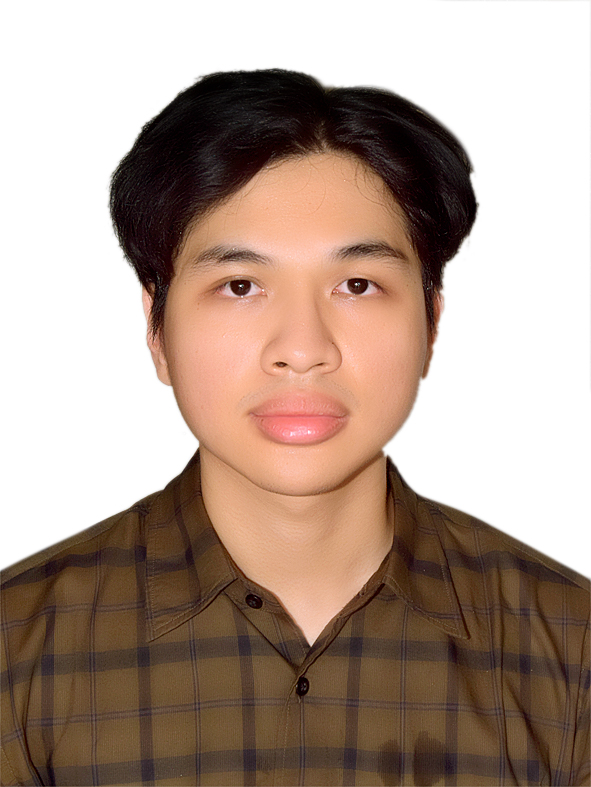
\includegraphics[height=4.5cm]{image/personal_image.jpg}}
\end{minipage}

\vspace{12mm}

% -----------------------------------------------------------------------------
% QUA TRINH DAO TAO -- start from undergraduate and work forward to the present.
% One \item per degree; keep the range separator (--) and terminal period.
% -----------------------------------------------------------------------------
\noindent\textbf{QUÁ TRÌNH ĐÀO TẠO} \textit{(Bắt đầu từ Đại học đến nay)}

\vspace{2mm}

\begin{itemize}[leftmargin=*, itemsep=2mm, topsep=0mm]
    \item Tháng 8/2018 -- Tháng 9/2022: Sinh viên, chuyên ngành Kỹ thuật Điều khiển và Tự động hóa, Trường Đại học Bách Khoa -- ĐHQG-HCM.
    \item Tháng 8/2023 -- Nay: Học viên cao học, chuyên ngành Khoa học Máy tính, Trường Đại học Bách Khoa -- ĐHQG-HCM.
\end{itemize}

\vspace{8mm}

% -----------------------------------------------------------------------------
% QUA TRINH CONG TAC -- start from your first job and work forward to the present.
% One \item per position; keep the range separator (--) and terminal period.
% -----------------------------------------------------------------------------
\noindent\textbf{QUÁ TRÌNH CÔNG TÁC} \textit{(Bắt đầu từ khi đi làm đến nay)}

\vspace{2mm}

\begin{itemize}[leftmargin=*, itemsep=2mm, topsep=0mm]
    \item Tháng 6/2022 -- Tháng 6/2026: Embedded Software Engineer tại công ty Bosch Global Software Technology Vietnam.
    \item Tháng 6/2026 -- Nay: Embedded Software Engineer tại công ty Hybrid Controls Vietnam Limited Company.
\end{itemize}


\end{document}
